\section{Data and Institutional Background}
\label{sec:data}

\subsection{DeFi liquidations as an observable deleveraging signal}

Decentralized lending protocols (Aave, Compound, Spark, Morpho, and related
systems) enforce collateralization rules through smart contracts. When a
borrower's collateral value relative to outstanding debt crosses a
protocol-defined threshold, any third party may repay part of the debt and
seize an equivalent amount of collateral at a discount. The event is
mechanical. It is triggered by price movement, not by borrower decision, and
under the fixed-spread designs of these protocols it settles on-chain within
a single block \citep{qin2021}. Each liquidation is
therefore an observable instance of forced deleveraging in the sense of
\citet{geanakoplos2010} and \citet{brunnermeier2009}: the object that
equilibrium credit models treat as a shadow quantity, the tightening of
collateral constraints, is here recorded transaction by transaction.

Two caveats qualify this observability at the outset. First, liquidator
behavior after seizure is not observed. Whether seized ETH is resold
immediately, consistent with the liquidator's incentive to realize the
bonus, or held instead, is a behavioral assumption, and the seized-collateral
measure is retained as a robustness alternative to the debt-repaid measure
used below. Second, the hourly aggregation imposed by the data source does
not resolve within-hour sequencing; the paper makes no claim about the order
of events inside a given hour.

\subsection{Panel and scope}

The dataset is an hourly UTC panel from 2021-03-15 00:00 to 2025-12-01 00:00
(exclusive), a raw grid of \NTotal{} hours with timestamps marking the start
of each bucket. Initializing rolling statistics consumes a \WarmupRows-hour
warmup, leaving an estimation panel of \Nobs{} hours. All sources are
public: Bybit (perpetual prices, open interest, funding), CCData spot
aggregates (ETH, BTC, and the placebo assets XRP and DOGE), Coinbase and
Binance feeds used for cross-venue audits, and Dune Analytics for on-chain
liquidations.

Two scope choices are deliberate. The hourly frequency is the
identification compromise. It is fine enough to separate a one-hour-ahead lead
from within-bucket simultaneity, and coarse enough that buckets carry
non-trivial liquidation mass. Daily aggregation would drown any cascade
dynamics, while tick-level sequencing is unavailable from the liquidation
source. The on-chain perimeter is an \emph{observability} constraint, not a
convenience. DeFi is the only segment where forced deleveraging is recorded
transaction by transaction. Liquidations on centralized derivatives
venues, where a reflexive spiral, if any, plausibly lives, cannot be
observed at this grain; they are neither tested nor refuted here
(Section~\ref{sec:discussion}). The window starts when joint coverage of
Bybit derivatives data and the Dune lending tables becomes adequate; the
sample is post--DeFi-Summer and excludes the March 2020 episode.

\subsection{The liquidation series}
\label{sec:data-liq}

Liquidations are extracted from Dune Analytics (query \texttt{6912877},
versioned in the replication package) over the open-source Spellbook tables
\texttt{lending.borrow} and \texttt{lending.supply}, covering all EVM chains
and lending protocols indexed at extraction time (Aave v1--v3, Compound
v2--v3, Spark, and Morpho account for the bulk of volume). The primary
measure is \emph{debt forcibly repaid}, in USD, aggregated by hour. This is
the leg that measures the deleveraging flow itself, how much leverage was
forcibly purged, rather than collateral seized, which mixes in the
liquidator's discount. \citet{perez2021} show that ninety-five percent of
liquidable collateral is liquidated within sixteen blocks, a few minutes at
most, which legitimates hourly aggregation: a liquidation is an event within
the hour, not a process spanning hours.

Four filters make the measure conservative and economically interpretable.
First, only liquidation-type events enter. Second, collateral is restricted to an
ETH-like whitelist (WETH, ETH, stETH, wstETH, rETH, cbETH, sfrxETH, ETHx),
with two caveats: liquid-staking derivatives are included, so the
collateral set is ETH-like in the broad sense; and the list predates the
liquid-restaking generation (weETH, ezETH, rsETH, osETH, and kin), which
became material lending collateral only in 2024--2025 and is therefore
absent. Because the collateral leg gates the join, this omission drops the
affected liquidations entirely, an under-count bounded below. Third, a dust filter (absolute
debt below \$5) removes a cluster of roughly 75{,}000 economically
immaterial bot-driven micro-events in September 2025. Fourth, exploit windows
are excluded (UwuLend from June 2024; Euler v1, March--April 2023), since
exploit-driven liquidations are endogenous to a hack, not to the market
cycle. Event tables are pre-aggregated by transaction before joining the
debt and collateral legs, eliminating a Cartesian-product inflation that
affects bundled liquidation transactions. Full query logic and exclusions
are documented in the data appendix.

Three structural omissions bound the interpretation. First, the source
aggregates to the hour: within-hour sequencing of prices and liquidations
is lost, so at short horizons the liquidation--return relation is
mechanically bidirectional. This is the basis for the paper's non-causal register
(Section~\ref{sec:stylized}). Second, MakerDAO, historically the largest
on-chain liquidator, sits outside the Spellbook lending schema (a CDP
architecture) and is de facto absent, so the measure understates total
on-chain deleveraging, most severely in 2021. Third, no
centralized-exchange liquidations enter: the shock is DeFi-only.

A direct check bounds what the MakerDAO omission can distort. We re-fit the
locked specification on a panel inflated by a missing-Maker mass (the
displacement figures below are the maximum over the defensible allocation
share $m \le 0.25$; extending the sweep to a punitive $m=0.5$ changes
neither sign nor significance),
allocated three economically credible ways: proportional to active
liquidations, concentrated in stress-adjacent hours, and weighted toward
high-leverage hours. The shock coefficient's sign stays intact under
every allocation, and the impact level moves by at most \MakerLevelImpactPct\%.
The level magnitude at \emph{medium} horizons is coverage-sensitive.
Under a leverage-weighted infill, the largest-displacement allocation, since
Maker liquidations cluster in high-leverage hours that are mechanically
correlated with the down tail, the twelve-hour deepening \emph{shrinks} by
as much as \MakerLevelMediumPct\%, so part of the apparent deepening is itself
a data-coverage artifact, compounding the overlap artifact of Section~\ref{sec:overlap}, rather than a property of the cycle. The object the paper's
conclusion rests on is more robust: the per-period exceedance asymmetry
$\Delta$ at the 1\% level (Section~\ref{sec:survives}) stays within
\MakerExcOverSesoi{} of the smallest effect size of interest under every
allocation, and moves \emph{toward} zero under the realistic ones, so
better Maker coverage would, if anything, sharpen the null. The full re-fit,
the three allocations, and the per-horizon displacements are reported in
Appendix~\ref{app:data}.

A second coverage gap operates the same way. The liquid-restaking tokens
that came to dominate leveraged ETH lending in 2024--2025 fall outside the
collateral whitelist, and because the collateral leg gates the join,
liquidations seizing only those tokens drop from the measure entirely. The
resulting under-count is one-sided and concentrated in the final third of the
sample, the same window in which the leverage-cycle interaction is identified.
As with the Maker omission, the direction is favorable: under-coverage of the
shock is attenuating measurement error in the regressor, biasing the
interaction and tail-asymmetry estimates toward the null the paper already
reports. One caveat resists this logic, and we flag rather than dismiss it:
restaking-token de-pegs (ezETH in April 2024, for instance) are not generic
deleveraging but sharp, clustered, downside events, so the missing mass may be
left-tail-selective rather than symmetric. On present evidence this does not
overturn the deconstruction, which rests on properties of the return
distribution and the estimator established independently of the shock's exact
magnitude (Sections~\ref{sec:deconstruction} and~\ref{sec:survives}); closing
it fully requires re-estimation on a collateral universe expanded to the
restaking generation, which we leave to future revision.

Total qualifying liquidations amount to \$\LiqTotalBn{} billion over the
sample. The flow is extremely sparse and right-skewed: \PLiqAll\% of
estimation-panel hours contain any liquidation; the mean daily flow is
\$\MeanDailyLiqM{} million against a median of \$\MedianDailyLiqK{}
thousand; and the largest single day (\$\MaxDayM{} million, 2024-08-05, the
yen carry-trade unwind) sits more than three orders of magnitude above the
median day (Figure~\ref{fig:timeseries}). These features motivate the
logarithmic shock transformation below. The external order of magnitude is
consistent with the \$2.49 billion over 42{,}324 liquidations that
\citet{lehar2022} report through mid-2022.

\subsection{Returns and market state}

The dependent variable is the hourly log return of the Bybit ETHUSDT
perpetual, $r_t = 100 \cdot \ln(P_t/P_{t-1})$. We select Bybit on a
cross-venue diagnostic: its return correlation with Binance perpetuals is
0.9989 and the mean absolute price spread is 1.98 basis points. We use the
perpetual rather than spot because crypto leverage lives in the perpetual,
matching a study of the leverage cycle. BTC spot returns serve a dual role:
they control for the dominant common crypto factor in the main
specification, and they form the basis of the orthogonalized placebo shock
(Section~\ref{sec:method}). Funding rate, the perpetual--spot basis, and
open interest describe the leverage state of the market; the high-leverage
regime indicator $\texttt{oi\_high}_t$ flags hours where open interest
exceeds its 80th rolling percentile over 720 hours. Open interest is
Bybit-only (the Binance series is a snapshot, not an hourly history), so the
leverage regime is measured at a single venue. We treat this as a
limitation. Finally, on-chain liquidations are triggered by oracle prices,
which are smoothed and partly CEX-anchored, so the trigger price is not
identical to the perpetual price being modeled. This oracle decoupling is
one mechanical reason liquidation--price feedback can be attenuated
\citep{caldarelli2020,liuszalachowski2021}.

\subsection{The shock variable}

The primary shock is the lagged log flow,
$L_{t-1} = \ln(1 + \text{liq}^{\text{USD}}_{t-1})$. The log tames a series
whose mean-to-median ratio exceeds two orders of magnitude; without it, a
handful of stress hours would mechanically dominate every regression. The
unit offset maps the roughly three-quarters of zero hours to zero while
remaining negligible against the post-filter minimum of \$5. The one-hour
lag means that ``$h=0$'' throughout the paper denotes a one-hour-ahead
prediction, which attenuates but does not eliminate within-bucket
simultaneity. The interaction $L_{t-1} \times \texttt{oi\_high}_t$ carries
the leverage-cycle amplification hypothesis. Timing conventions, the
raw-versus-orthogonalized shock architecture, and the identification logic
are in Section~\ref{sec:method}.

\subsection{Descriptive statistics}

Table~\ref{tab:descriptives} reports the estimation-panel descriptives:
return moments for ETH and BTC (Panel A) and the tail-asymmetry and
liquidation co-occurrence measures (Panel B) that anchor the stylized facts
of the next section. All entries are computed by a single re-executable
script from the canonical panel.

\begin{table}[t]
\centering
\caption{Descriptive statistics, estimation panel (hourly, 2021--2025).}
\label{tab:descriptives}
% GENERATED by scripts/paper/make_tables.py — DO NOT EDIT
% fragment only: wrap in \begin{table} + caption in the manuscript
\begin{tabular}{lcc}
\toprule
 & ETH perp & BTC spot \\
\midrule
\multicolumn{3}{l}{\emph{Panel A: hourly log-returns (\%)}} \\
$N$ (hours) & 40,582 & 40,582 \\
Mean & 0.0005 & 0.0009 \\
Std.\ dev. & 0.812 & 0.609 \\
Skewness & -0.628 & -0.369 \\
Excess kurtosis & 17.6 & 15.0 \\
Min & -15.46 & -10.92 \\
$p_{1}$ & -2.46 & -1.86 \\
$p_{99}$ & 2.33 & 1.80 \\
Max & 9.17 & 6.24 \\
\midrule
\multicolumn{3}{l}{\emph{Panel B: tail asymmetry and liquidation co-occurrence (ETH)}} \\
\#\{$r \le -5\%$\} / \#\{$r \ge +5\%$\} & \multicolumn{2}{c}{50 / 25} \\
\#\{$r \le -7\%$\} / \#\{$r \ge +7\%$\} & \multicolumn{2}{c}{13 / 6} \\
$|p_{1}|/p_{99}$ (quantile ratio) & \multicolumn{2}{c}{1.05} \\
$P(\text{liq}>0 \mid \text{worst 1\% hours})$ & \multicolumn{2}{c}{85.5\%} \\
$P(\text{liq}>0 \mid \text{best 1\% hours})$ & \multicolumn{2}{c}{41.6\%} \\
$P(\text{liq}>0)$ (all hours) & \multicolumn{2}{c}{27.0\%} \\
\bottomrule
\end{tabular}

\begin{minipage}{0.92\textwidth}
\vspace{2pt}
{\scriptsize \emph{Notes:} Hourly log returns in percent; $N=\Nobs$
(\NTotal{} raw hours less a \WarmupRows-hour rolling-window warmup).
Far-extreme counts are inclusive threshold counts on returns in percent.
The co-occurrence rows condition on the within-sample 1\% return quantiles
and use contemporaneous liquidations ($\text{liq}_t > 0$). Source:
\texttt{descriptive\_stats.csv}, generated by
\texttt{run\_descriptive\_stats.py}.}
\end{minipage}
\end{table}

\begin{figure}[t]
\centering
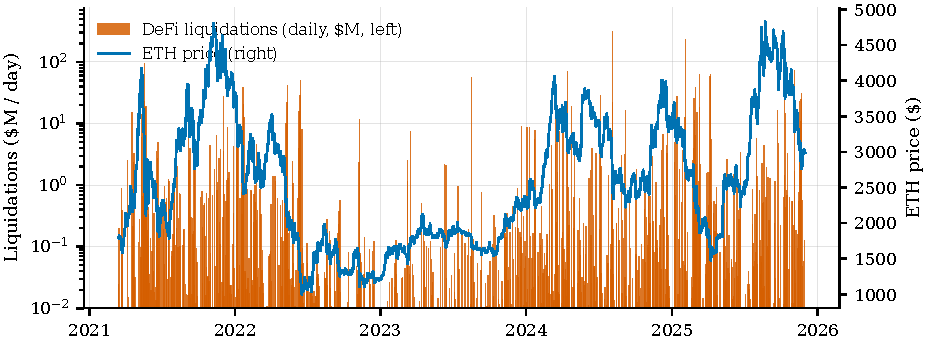
\includegraphics[width=\textwidth]{../paper/figures/fig1_liquidations_timeseries}
\caption{Daily DeFi liquidations (ETH-like collateral, log scale) and the
ETH price, 2021--2025. The flow is sparse, right-skewed, and concentrated
in a handful of stress episodes.}
\label{fig:timeseries}
\end{figure}

\subsection{Data limitations}
\label{sec:data-limits}

The data limitations flagged above are collected here in one place: (1)
hourly aggregation, hence lost within-hour sequencing and short-horizon
bidirectionality; (2) MakerDAO de facto absent; (3) no centralized-exchange
liquidations; (4) ETH-like collateral includes liquid-staking derivatives
but predates and so excludes the liquid-restaking generation, a one-sided
under-count concentrated in 2024--2025;
(5) open interest and funding measured at a single venue; (6) BTC--ETH
co-movement implies the shock is partly a common-crypto stress proxy
(Sections~\ref{sec:deconstruction} and~\ref{sec:discussion}); (7) turnover
denominators used for scale comparisons are industry estimates, partly
inflated by wash trading, and are treated as order-of-magnitude bounds only,
since the liquidation numerator is the only hard number; (8) the window is
post--DeFi-Summer; (9) the dust and exploit filters make the measure
conservative.